
\documentclass[12pt]{article}
%	options include 12pt or 11pt or 10pt
%	classes include article, report, book, letter, thesis
\usepackage{graphicx}
\usepackage[useregional]{datetime2}
\usepackage{caption}

\author{Adam Blance 40161070}
\begin{document}

	\title{SET10108 Concurrent and Parallel Systems \linebreak Coursework 2 \linebreak N-Body Simulation}
	\markboth{40161070}{}
	\maketitle
\begin{abstract}
In this paper the task was to solve the N-Body problem using several paralleiziation techniques. To complete this task the two approaches used were OpenMP and CUDA this allowed for a direct comparison of the GPU and CPU. These were measured in two different ways, these being time taken to complete the simulation and the frame rate the application achieved during the run time. These results were the displayed in tables and discussed. Proving that paralleiziation is faster on the GPU, although paralleiziation on the CPU is simpler.
		
\end{abstract}
\begin{figure}
	\centering
	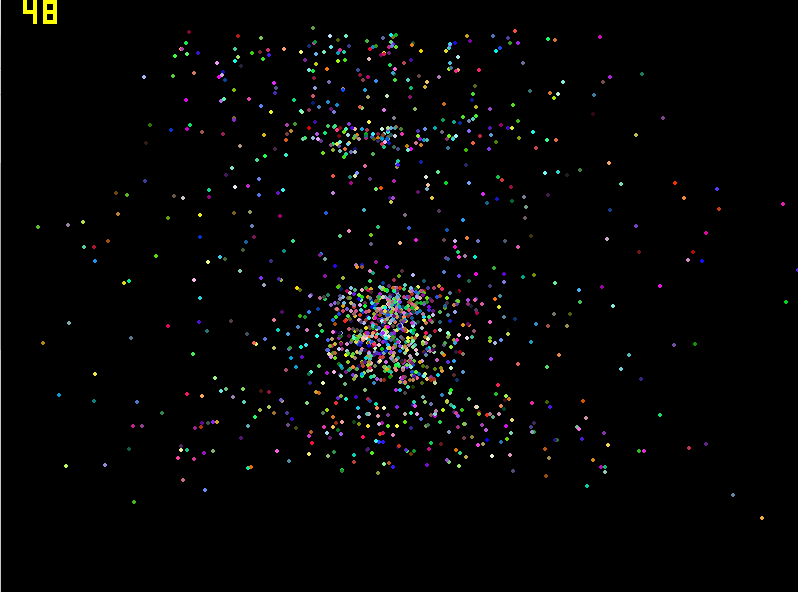
\includegraphics[scale=0.5]{pics/intro.png}
	\caption{An N-Body simulation.}
\end{figure}
\newpage 		
\section{Introduction}
As more and more of our world becomes heavily reliant on data found online, it is  becoming more necessary to learn how to parallelize this data, allowing data to be processed as quickly as possible.  Learning how to parallelize sequential systems has become a very important skill to possess in your repertoire. 
\newline 
In this course-work the task was to parallelize an N-body algorithm. An N-Body algorithm is a simulation where a particle is affected by the all other particles according to the laws of physics. Issues occur when large amounts of particles are rendered on the screen. This causes any program running an N-Body simulation sequentially to struggle. This is known as the N-Body problem. In this report several
parallelization techniques were used to solve the N-Body problem and compared.

\section{Inital Analysis}
The first task in the course work was choosing which of the three tasks posed to us. It was decided that N-Body simulation would be the task that would be selected. The reason for deciding on N-Body simulation was because research into JPEG compression found little results and while prime numbers search was possible, N-body was chosen down to personal preference.
\newline 
Once this was decided on research was conducted into N-Body simulation and which algorithm online would be used to parallelise. During the search many possible candidates were found but the best one was harrism/mini-nbody . The reason for this was it because of its relative simplicity allowing for graphical output to be easily added into the code. After that small tweaks were made to the N-Body simulation and using Allegro 5, a graphical interface was created. From this point the initial analysis was conducted.
\subsection{First Results}
It was decided that 3 things would be tested to gather the baseline data of the application to discover any bottlenecks. These were:
\begin{itemize}
 \item Length of Simulation.
 \item Size of Times Step.
  \item Number of Particles. 
\end{itemize}
These three factors were measured by the execution time, this was calculated by taking using the system clock and printed to a console, also taken was the average framerate this was measured using Fraps. The tables for the measurements are shown below.
\subsubsection{Length of Simulation}
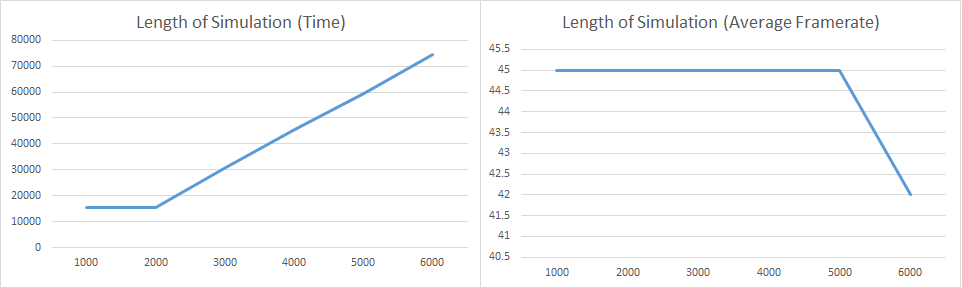
\includegraphics[scale=0.5]{pics/ialength.png}
\newline
The reason for measuring the length of the simulation was to see if a drop off occurred at any point and performance suffered because of this. This was measured in number of iterations. As shown in the results no bottleneck occurred at any point as the time taken increased at steady amount as was expected and the framerate did not suffer at all. An anomaly occurred during this test. This being the framerate dropping to 42 fps rather the holding at 45 fps like the other tests this probably had nothing to do with code and with assumed to be an anomaly. The other strange occurrence in this test was that ///comeback to this /////
\subsubsection{Size of Times Step}
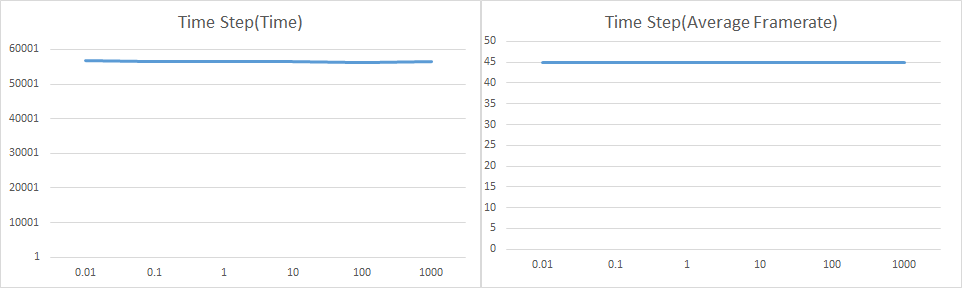
\includegraphics[scale=0.5]{pics/iatime.png}
\newline

\subsubsection{ Number of Particles}
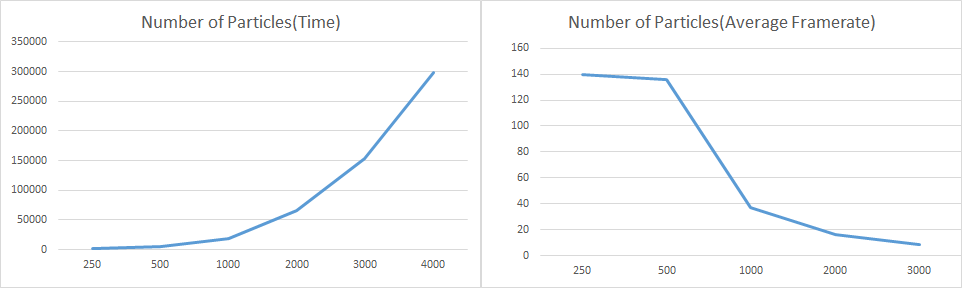
\includegraphics[scale=0.5]{pics/ianumber.png}
\newline
The final measurement that was taken was Number of Particles the graph show clearly that a bottleneck occurs as the number of particles increases, this is because increasing the number of particles increases the number of calculations the PC must perform exponentially. The aforementioned test clearly states the place that must be parallelized. The code that will be parallelized is shown below.
////////put in code/////// 
\newline
	
\section{Methodology}
To solve the bottle-neck that was defined in the initial analysis several parallelization techniques were used. These were OpenMP and CUDA. The idea behind using these approaches was to be able to compare parralelization on the GPU against  parralelization on the CPU.They would be measured by increasing the number of particles on screen and their results would be presented below.
\newline
To keep the values constant each test was run 11 times and an average value was calculated with the first value being ignored to allow the program to warm up. Another step that was taken to keep consistency between results was to keep the hardware constant on all tests. The hardware was:
\begin{itemize}
	\item soomeibnga
	\item S
	\item te
\end{itemize}
 To evaluate these techniques two values were quantified, these being the time taken to complete the simulation and the average frame-rate. To calculate the time taken this system clock within Visual Studio was used. This was important to present in the results as it is the most common and easiest way to compare with a sequential program. To measure the Frame-rate Fraps was used. The reason for this is because in most simulations the frame-rate is more important then the time taken. 

\subsubsection{OpenMP}
The first approach was to use OpenMP, OpenMP is a library to support shared memory concurrency that works in the CPU, allowing it to be portable and added easily to the program. It can  be easily used in conjunction with other approaches allowing more threading to be added at a later stage.
\newline 
To implement OpenMP was fairly straight forward as the bottleneck had already been identified in the initial analysis. As OpenMP deals very well with for loops the code was very simple to apply to the application.
\subsubsection{CUDA}
CUDA is a  parallel computing platform and application programming interface model created by Nvidia. It works inside the GPU to allow for great speed-up potential. CUDA was designed to work with programming languages such as C and C++ which makes it easier to use as a product compared to other APIs. Its use of shared and unified memory, which allows multiple programs to use the same memory.
\newline
 To carry out the task of adding CUDA to the application, a different approach was taken as CUDA is more complicated to add then OpenMP. Once CUDA was installed in Visual Studio it was discovered that the code would have to be completely reworked to add CUDA into the programme. This may not have been the case but a lack of overall knowledge in the background of CUDA restricted the outcome of the project.
 \newline 
 The place that the parrelization was to be added would be the same place as OpenMP however before this could be implemented the code needed to be converted to a kernal.

\section{Results}

\section{Conclusion}


	
\end{document}